\documentclass[10pt,openright,twoside,french]{book}

\input philippe2013
\input philippe2013_cours
\input philippe2013_sections
\input philippe2013_chapitre


\begin{document}

\chapter[\'Equations et inéquations]{\'Equations et inéquations\\ Résolution de problèmes}\label{ch_equation}

\section{Résolution d'équations}
\subsection{Développement et factorisation}

\begin{Defi}
    \iptb{Développer}\index{développement} un produit revient à l'écrire sous forme d'une somme.
\end{Defi}

\begin{Prop}[(démontrée pour les nombres positifs à l'aide de la géométrie en exercice)]
    Pour tous nombres $k$, $a$, $b$, $c$ et $d$, on a :
    \[k(a + b) = ka + kb \qetq (a + b)(c + d) = ac + ad + bc+ bd.\]
\end{Prop}

\begin{Exemple}
    Développer l'expression $A(x) = 5(x - 1) - (3x - 2)(-4 + x)$.\par\smallskip
    \hspace{-2cm}$\begin{array}{r@{\ =\ }ll}
        A(x) & 5(x - 1) - (3x - 2)(-4 + x) & \\[7pt]
        A(x) & 5x - 5 - (3x - 2)(-4 + x) & \rightsquigarrow\ \text{on commence par développer} \\[7pt]
        A(x) & 5x - 5 -(-12x + 3x^2 + 8 - 2x) & \rightsquigarrow\ \text{attention aux signes !}\\[7pt]
        A(x) & 5x - 5 + 12x - 3x^2 - 8 + 2x & \rightsquigarrow\ \text{suppression de la parenthèse}\\[7pt]
        A(x) & -3x^2 + 5x + 12x + 2x - 8 & \rightsquigarrow\ \text{puis réduction de l'expression} \\[7pt]
        \multicolumn{3}{l}{\pfr{A(x) = -3x^2 + 19x - 8}}
    \end{array}$
\end{Exemple}

\begin{Defi}
    \iptb{Factoriser}\index{factorisation} une somme revient à l'écrire sous forme d'un produit.
\end{Defi}

\begin{Prop}[(démontrée pour les nombres positifs à l'aide de la géométrie en exercice)]
    Pour tous nombres $k$, $a$, $b$, $c$ et $d$, on a :
    \[ka + kb = k(a + b) \qetq a(c + d) + b(c + d) = (a + b)(c + d).\]
\end{Prop}

\begin{Exemple}
    Factoriser l'expression $B(x) = 2(x+4)+2(x-1) - (2x + 3)(4x + 6)$.\par\smallskip
    \hspace{-2cm}$\begin{array}{r@{\ =\ }ll}
        B(x) & \textcolor{red}{2}(x+4)+\textcolor{red}{2}(x-1) - (2x + 3)(4x + 6) & \rightsquigarrow\ \text{on repère les facteurs communs} \\[7pt]
        B(x) & 2(x + 4 + x - 1) - (2x + 3)(4x + 6) & \rightsquigarrow\ \text{pas de problème de signes avec un $+$} \\[7pt]
        B(x) & 2\textcolor{red}{(2x + 3)} - \textcolor{red}{(2x + 3)}(4x + 6) & \rightsquigarrow\ \text{on continue tant qu'il y a un facteur commun}\\[7pt]
        B(x) & (2x + 3)(2 - (4x + 6)) & \rightsquigarrow\ \text{attention au signe $-$} \\[7pt]
        B(x) & (2x + 3)(2 - 4x - 6) & \rightsquigarrow\ \text{suppression de la parenthèse} \\[7pt]
        B(x) & (2x + 3)(\textcolor{red}{-4} + \textcolor{red}{-4}x) & \rightsquigarrow\ \text{il y a encore un facteur commun} \\[7pt]
        \multicolumn{3}{l}{\pfr{B(x) = -4(2x + 3)(1 + x)}}
    \end{array}$
\end{Exemple}
\clearpage

\begin{Prop}[Les identités remarquables]
    Soient $a$ et $b$ deux nombres quelconques. On a alors les \ipt{identités remarquables} suivantes :
    \begin{center}
    \begin{tabular}{rcl}
        \underbar{Forme factorisée} && \underbar{Forme développée} \\[7.5pt]
        $(a + b)^2$ & $=$ & $a^2 + 2ab + b^2$ \\
       $(a - b)^2$ & $=$ & $a^2 - 2ab + b^2$ \\
        $(a + b)(a - b)$ & $=$ & $a^2 - b^2$
    \end{tabular}
    \end{center}
\end{Prop}

\begin{Demo}
    \[\begin{array}[c]{rcl}
        (a + b)^2 & = & (a + b)(a + b) \\
                         & = & a^2 + ab + ba + b^2\\
                         & = & a^2 + ab + ab + b^2 \\
        \multicolumn{3}{l}{\pfr{(a + b)^2 = a^2 + 2ab + b^2}}
    \end{array} \qq
    \begin{array}[c]{rcl}
        (a - b)^2 & = & \big(a + (- b)\big)^2 \\
                        & = & a^2 + 2 \times a \times (-b) + (-b)^2\\
        \multicolumn{3}{l}{\pfr{(a - b)^2 = a^2 - 2ab + b^2}}
      \end{array}\]

    \[\begin{array}[t]{rcl}
            (a + b)(a - b) & = & a^2 - ab + ba - b^2\\
                                   & = & a^2 - ab + ab + b^2 \\
            \multicolumn{3}{l}{\pfr{(a + b)(a - b) = a^2 - b^2}}
    \end{array}\]
\end{Demo}\medskip

\begin{Exemple}[s]
    $\begin{array}[t]{rcl}%
        C & = & 1\,001^2 \\
        C & = & (1\,000 + 1)^2 \\
        C & = & 1\,000^2 + 2 \times 1\,000 \times 1 + 1^2\\
        C & = & 1\,000\,000 + 2\,000 + 1 \\
        \multicolumn{3}{l}{\pfr{C = \NP{1002001}}}
    \end{array}$
    $\begin{array}[t]{rcl}%
        D & = & 99^2 \\
        D & = & (100 - 1)^2 \\
        D & = & 10\,000 - 200 + 1 \\
        \multicolumn{3}{l}{\pfr{D = \NP{9801}}}
    \end{array}$
    $\begin{array}[t]{rcl}%
        E & = & 49 \times 51 \\
        E & = & (50 - 1)(50 + 1) \\
        E & = & 50^2 - 1^2 \\
        E & = & 2\,500 - 1 \\
        \multicolumn{3}{l}{\pfr{E = \NP{2499}}}
    \end{array}$
\end{Exemple}\medskip
%
\begin{Exemple}[s]
    $\begin{array}[t]{rcl}
        F(x) & = & x^2 + 2x + 1 \\
        F(x) & = & x^2 + 2 \times x \times 1 + 1 \\
        \multicolumn{3}{l}{\pfr{F(x) = (x + 1)^2}}
    \end{array}$
    $\begin{array}[t]{rcl}
        G(a) & = & 9a^2 - 24a + 16 \\
        G(a) & = & 9a^2 - 2 \times 12x + 16 \\
        G(a) & = & (3a)^2 - 2 \times 3a \times 4 + 4^2\\
        \multicolumn{3}{l}{\pfr{G = (3a - 4)^2}}
    \end{array}$
    $\begin{array}[t]{rcl}
        H(y) & = & y^2 - 25 \\
        H(y) & = &  y^2 - 5^2\\
        \multicolumn{3}{l}{\pfr{H(y) = (y - 5)(y + 5)}}
    \end{array}$
\end{Exemple}\medskip

\begin{Rmq}
    Les identités remarquables sont utiles pour gagner du temps dans un développement et, en cas d'oubli, on peut les retrouver en quelques lignes.\par
    En revanche, elles sont très pratiques pour factoriser dans certains cas où il n'y a pas de facteurs communs.
\end{Rmq} \medskip

\begin{Exemple}
    On désire factoriser $I(t) = 4t^2 - 20t + 9$.\par
    On écrit alors $I(t)$ de la manière suivante : \[I(t) = (2t)^2 - 2 \times 2t \times 5 + 3^2\] mais la forme obtenue ne nous convient pas. Comment faire ?\par
    \textit{Indication :} $9 = 25 - 16 = 5^2 - 4^2$.
\end{Exemple}

\subsection{Les équations}

\begin{Defi}
    Une \iptb{équation}\index{equation@équation} est une égalité où figure une inconnue.\par
    \iptb{Résoudre} une équation revient à trouver la (ou les) valeur(s) de l'inconnue pour laquelle (ou lesquelles) l'égalité est vérifiée.
\end{Defi}\clearpage

\begin{Prop}
On peut ajouter un même nombre à chaque membre d'une égalité pour obtenir ainsi une égalité équivalente :
    \[a = b \qLRq a \rouge{\ +\ c } = b \rouge{\ +\ c}\]
\end{Prop}

\begin{Demo}
    Puisque $a = b$ alors $a - b = 0$ et puisque $c - c = 0$, on a :
    \[0 = a - b + c - c = a + c - b - c = a + c - (b + c) = 0 \quad \text{donc} \quad a+c = b+c.\]
\end{Demo}

\begin{Prop}
    On peut multiplier par un même nombre non nul les deux membres d'une égalité pour obtenir ainsi une égalité équivalente :
    \[\text{Avec } c\neq 0,\quad a = b \qLRq a \rouge{\,\times\,c} = b \rouge{\,\times\,c}\]
\end{Prop}

\begin{Demo}
    Puisque $a = b$ alors $a - b = 0$ et puisque $c \neq 0$, on a :
    \[0 = c(a - b) = ca - cb = 0 \quad \text{donc} \quad a \times c = b \times c.\]
\end{Demo}

\subsubsection{\'Equation du premier degré}
\begin{Defi}
    Une \iptb{équation à une inconnue du premier degré}\index{equation@équation!équation du premier degré} est une équation de la forme $ax + b = 0$ où $x$ est l'inconnue et $a$ et $b$ sont des paramètres donnés tels que $a \neq 0$.\par
\end{Defi}

\begin{Exemple}
    Résolution de l'équation : $8x - 3 = -2x + 6$.\par\smallskip
    $\begin{array}{r@{\qLRq}ll}
        8x - 3 = -2x + 6 & 8x - 3 ~\rouge{+2x} = -2x + 6 ~\rouge{+2x} & \rightsquigarrow\ \text{on regroupe l'inconnue d'un seul côté} \\[7pt]
         &   10x - 3 ~\rouge{+3} = 6 ~\rouge{+3} &\rightsquigarrow\ \text{on isole l'inconnue} \\[7pt]
        & 10x ~\rouge{\div 10} = 9 ~\rouge{\div 10} & \\[7pt]
        & \pfr{x = \frac{9}{10} = 0,9} &
    \end{array}$\medskip

    Le nombre $0,9$ est la solution de l'équation.
\end{Exemple}\medskip

\begin{Exemple}[s]
    Résoudre les équations suivantes :
    \[3x - 4 = 3 \qq 2x + 2 = 5x - 4 \qq 1 - 2(2 - x) = 2x - 3\]
\end{Exemple}

\subsubsection{\'Equation produit}\index{equation@équation!équation produit}
\begin{Prop}[(admise)]
    Un produit de facteur est nul si et seulement si l'un des facteurs est nul :
    \[A(x) \times B(x) = 0 \qLRq A(x) = 0 \text{ ou } B(x) = 0\]
\end{Prop}\clearpage

\begin{Exemple}
    Résolution de l'équation $(2x + 3)(6x - 8) = 0$.\par\smallskip

    Un produit de facteur est nul si et seulement si l'un des facteurs est nul donc :\smallskip

    \hspace{-1cm}$\begin{array}{r@{\qLRq}ll}
        (2x + 3)(6x - 8) = 0 & 2x+3 = 0 \text{ ou } 6x - 8 = 0 & \rightsquigarrow\ \text{on applique la propriété} \\[7pt]
         &   2x = -3 \text{ ou } 6x = 8 &\rightsquigarrow\ \text{équations du premier degré} \\[7pt]
        & x = -\frac 3 2 \text{ ou } x = \frac 8 6 = \frac 43 & \rightsquigarrow\ \text{on écrit les fractions sous forme irréductible} \\[7pt]
    \end{array}$

    \textbf{Les} solutions de l'équation sont donc $-\frac 3 2$ et $\frac 43$.
\end{Exemple}

\subsubsection{Résolution d'un problème}
\begin{Exemple}
    Lors d'une séance de cinéma, on a accueilli $56$ spectateurs. Certains ont payé le tarif réduit (\EUR{$5$}), les autres le tarif normal (\EUR{$8$}). La recette de cette séance se monte à \EUR{$376$}.\par Combien de spectateurs ont payé le tarif réduit ? (réponse : $24$)
\end{Exemple}

Voici les étapes de la résolution d'un problème en utilisant les équations :
\begin{enumerate}
    \item choix de l'inconnue ;
    \item mise en équation du problème ;
    \item résolution de l'équation ;
    \item réponse au problème.
\end{enumerate}\medskip


\section{Les ensembles de nombres en résumé}

\begin{Defi}
    \begin{enumerate}
        \item L'ensemble des entiers \ipt{naturels}\index{ensemble de nombres!entiers naturels} $\N$ est constitué des nombres entiers positifs.\par
        \item L'ensemble des entiers \ipt{relatifs}\index{ensemble de nombres!entiers relatifs} $\Z$ est constitué des entiers naturels ainsi que de nombres entiers négatifs.\par
        \item L'ensemble des nombres \ipt{rationnels}\index{ensemble de nombres!nombres rationnels} $\Q$ est constitué de tous les nombres qui peuvent s'écrire sous forme de fractions, ce qui inclut les ensembles $\N$ et $\Z$ mais aussi les nombres décimaux.\par
        \item L'ensemble des nombres \ipt{irrationnels}\index{ensemble de nombres!nombres irrationnels} est constitué des nombres qui ne peuvent pas s'écrire sous forme de fractions.
        \item L'ensemble des nombres \ipt{réels}\index{ensemble de nombres!nombres réels} $\R$ est constitué de tous les nombres rationnels et des nombres irrationnels.
    \end{enumerate}
\end{Defi}\medskip

\begin{center}
\pfr{$\N \subset \Z \subset \Q \subset R$}\medskip

\begin{tikzpicture}[scale=0.75]
    \fill[color=magenta!20] (0,0) ++(35:3.5) circle (4); % R
        \draw (0,0) ++(35:3.5) circle (4); % R
        \draw (0,0) node{$\R$};
    \fill[color=midblue!20] (0,0) ++(30:3.5) circle (2.75); % Q
        \draw (0,0) ++(30:3.5) circle (2.75); % Q
        \draw (3.2,0) node{$\Q$};
    \fill[color=orange!20] (0,0) ++(35:4) circle (1.75); % Z
        \draw (0,0) ++(35:4) circle (1.75); % Z
        \draw (4,3) node{$\Z$};
    \fill[color=OliveGreen!20] (0,0) ++(35:3.5) circle (0.75); % N
        \draw (0,0) ++(35:3.5) circle (0.75); % N  
        \draw (2.5,2) node{$\N$};
    \begin{scriptsize}
        \draw(2.9,2.5) node{$0$}; \draw(3.2,1.75) node{$23$};
        \draw(2.5,3.5) node{$-2$}; \draw(4.5,2.05) node{$-10$};
        \draw(1,2.5) node{$6,4$}; \draw(1.5,0.5) node{$\frac 13$}; \draw(5,0.75) node{$-\frac 47$};
        \draw(-0.5,3.25) node{$2\pi$}; \draw(3,5.5) node{$-\sqrt 7$};
    \end{scriptsize}
\end{tikzpicture}
\end{center}

\section{Résolution d'inéquations}
\subsection{Intervalles de nombres}\index{intervalles}
\subsubsection{Intervalles bornés}
\begin{Defi}
    Un \iptb{intervalle borné} par deux nombres réels est constitué de tous les nombres réels compris entre ces deux nombres.\par
    Par exemple, l'intervalle $\intervalleff  a b$ est l'ensemble des nombres $x$ tels que $x \geq a$ et $x \leq b$.
\end{Defi}

\begin{center}
\begin{tabular}{|>\bfseries c|>\bfseries c|>\bfseries m{7cm}|}
    \hline
        Inégalité & Notation & Représentation \\
    \hline
        $a \leq x \leq b$ & $x\in \intervalleff a b$ &
    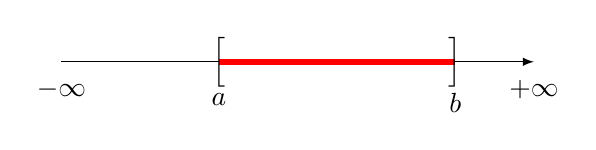
\begin{tikzpicture}[>=latex]
    \draw[->] (0,0) --(6,0);
    \draw[line width=2pt,color=red] (2,0)--(5,0);
    \node[] at (5,0) {\rouge{$\Big]$}};
    \node[] at (2,0) {\rouge{$\Big[$}};
    \node[below=8pt] at (5,0) {$b$};
    \node[below=3pt] at (0,0) {$-\infty$};
    \node[below=3pt] at (6,0) {$+\infty$};
    \node[below=8pt] at (2,0) {$a$};
\end{tikzpicture}\\
\hline
        $a < x \leq b$ & $x\in \intervalleof a b$ &
    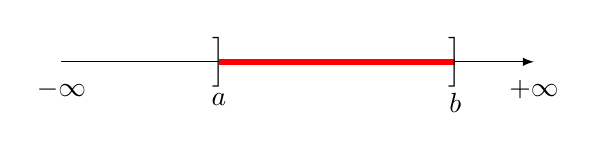
\begin{tikzpicture}[>=latex]
    \draw[->] (0,0) --(6,0);
    \draw[line width=2pt,color=red] (2,0)--(5,0);
    \node[] at (5,0) {\rouge{$\Big]$}};
    \node[] at (2,0) {$\Big]$};
    \node[below=8pt] at (5,0) {$b$};
    \node[below=3pt] at (0,0) {$-\infty$};
    \node[below=3pt] at (6,0) {$+\infty$};
    \node[below=8pt] at (2,0) {$a$};
\end{tikzpicture}\\
\hline
        $a \leq x < b$ & $x\in \intervallefo a b$ &
    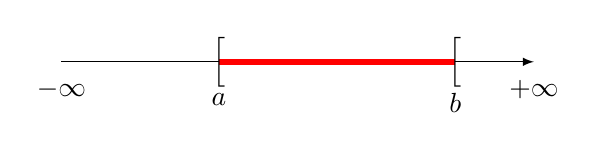
\begin{tikzpicture}[>=latex]
    \draw[->] (0,0) --(6,0);
    \draw[line width=2pt,color=red] (2,0)--(5,0);
    \node[] at (5,0) {$\Big[$};
    \node[] at (2,0) {\rouge{$\Big[$}};
    \node[below=8pt] at (5,0) {$b$};
    \node[below=3pt] at (0,0) {$-\infty$};
    \node[below=3pt] at (6,0) {$+\infty$};
    \node[below=8pt] at (2,0) {$a$};
\end{tikzpicture}\\
\hline
        $a < x < b$ & $x\in \intervalleoo a b$ &
    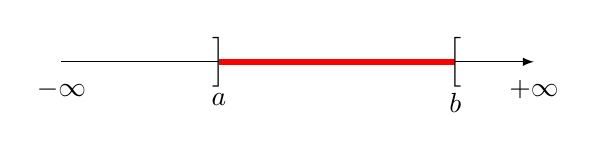
\begin{tikzpicture}[>=latex]
    \draw[->] (0,0) --(6,0);
    \draw[line width=2pt,color=red] (2,0)--(5,0);
    \node[] at (5,0) {$\Big[$};
    \node[] at (2,0) {$\Big]$};
    \node[below=8pt] at (5,0) {$b$};
    \node[below=3pt] at (0,0) {$-\infty$};
    \node[below=3pt] at (6,0) {$+\infty$};
    \node[below=8pt] at (2,0) {$a$};
\end{tikzpicture}\\
\hline
\end{tabular}
\end{center}

\subsubsection{Intervalles non bornés}
\begin{Defi}
    Un \iptb{intervalle non borné} est constitué de tous les nombres réels supérieurs ou inférieurs à un nombre réel.\par
    Par exemple, l'intervalle $\intervalleoo{a}{+\infty}$ est l'ensemble des nombres $x$ tels que $x > a$.
\end{Defi}

\begin{center}
\begin{tabular}{|>\bfseries c|>\bfseries c|>\bfseries m{7cm}|}
    \hline
        Inégalité & Notation & Représentation \\
    \hline
        $x \geq a $ & $x\in \intervallefo{a}{+\infty}$ &
    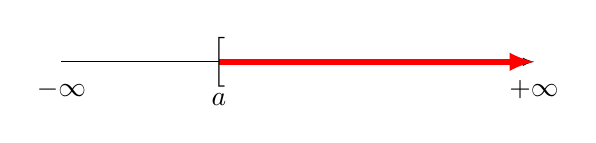
\begin{tikzpicture}[>=latex]
    \draw[->] (0,0) --(6,0);
    \draw[line width=2pt,color=red,->] (2,0)--(6,0);
    \node[] at (2,0) {\rouge{$\Big[$}};
    \node[below=3pt] at (0,0) {$-\infty$};
    \node[below=3pt] at (6,0) {$+\infty$};
    \node[below=8pt] at (2,0) {$a$};
\end{tikzpicture}\\
\hline
        $x > a $ & $x\in \intervalleoo{a}{+\infty}$ &
    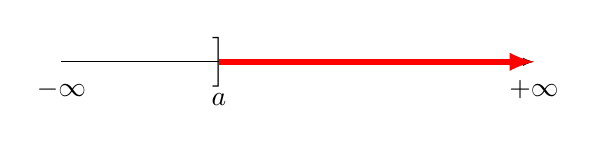
\begin{tikzpicture}[>=latex]
    \draw[->] (0,0) --(6,0);
    \draw[line width=2pt,color=red,->] (2,0)--(6,0);
    \node[] at (2,0) {{$\Big]$}};
    \node[below=3pt] at (0,0) {$-\infty$};
    \node[below=3pt] at (6,0) {$+\infty$};
    \node[below=8pt] at (2,0) {$a$};
\end{tikzpicture}\\
\hline
        $x \leq a $ & $x\in \intervalleof{-\infty}{a}$ &
    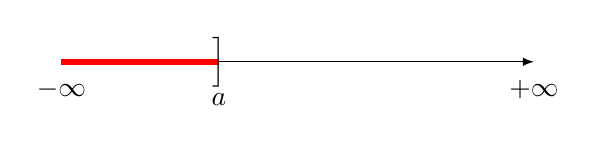
\begin{tikzpicture}[>=latex]
    \draw[->] (0,0) --(6,0);
    \draw[line width=2pt,color=red] (0,0)--(2,0);
    \node[] at (2,0) {\rouge{$\Big]$}};
    \node[below=3pt] at (0,0) {$-\infty$};
    \node[below=3pt] at (6,0) {$+\infty$};
    \node[below=8pt] at (2,0) {$a$};
\end{tikzpicture}\\
\hline
        $x < a $ & $x\in \intervalleoo{-\infty}{a}$ &
    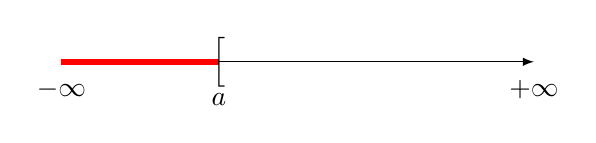
\begin{tikzpicture}[>=latex]
    \draw[->] (0,0) --(6,0);
    \draw[line width=2pt,color=red] (0,0)--(2,0);
    \node[] at (2,0) {{$\Big[$}};
    \node[below=3pt] at (0,0) {$-\infty$};
    \node[below=3pt] at (6,0) {$+\infty$};
    \node[below=8pt] at (2,0) {$a$};
\end{tikzpicture}\\
\hline
\end{tabular}
\end{center}

\subsubsection{Réunion et intersection}
\begin{Defi}
    \begin{enumerate}
        \item La \ipt{réunion} de deux intervalles $I$ et $J$, notée $I \cup J$, est l'ensemble des nombres réels appartenant à $I$ \textbf{ou} à $J$.
        \item L'\ipt{intersection} de deux intervalles $I$ et $J$, notée $I \cap J$, est l'ensemble des nombres réels appartenant à $I$ \textbf{et} à $J$.
    \end{enumerate}
\end{Defi}

\begin{Exemple}[s]
$\intervalleff{-2}{5} \cup \intervalleoo{0}{+\infty} = \intervallefo{-2}{\infty} \qq \intervalleff{-2}{5} \cap \intervalleoo{0}{+\infty} = \intervalleof 0 5$ \medskip

$\intervalleff{-2}{5} \cup \intervalleof{8}{15} = \intervalleff{-2}{5} \cup \intervalleof{8}{15}$ (on ne peut pas écrire la réunion sous forme d'un seul intervalle).\medskip

$\intervalleff{-2}{5} \cap \intervalleof{8}{15} = \emptyset$ (ensemble vide) : l'intersection ne contient aucun nombre.
\end{Exemple}\medskip

\begin{Rmq}
    On a les inclusions suivantes :
    \[I \subset I \cup J \qq J \subset I \cup J \qq I \cap J \subset I \qetq I \cap J \subset J.\]
\end{Rmq}

\subsection{Résolution d'inéquations}
\subsubsection{Inéquations du premier degré à une inconnue}

\begin{Prop}
    On peut ajouter un même nombre à chaque membre d'une inégalité pour obtenir ainsi une inégalité équivalente :
    \[a < b \qLRq a \rouge{\ +\ c } < b \rouge{\ +\ c}\]
\end{Prop}

\begin{Exemple}[s]
    $\begin{array}[t]{rcl}
        x + 4 & \leqslant & 5 \\
        x + 4 \rouge{\,-\,4} & \leqslant & 5 \rouge{\,-\,4} \\
        \multicolumn{3}{c}{\pfr{x\leqslant 1}}
    \end{array}$\quad
    $\begin{array}[t]{rcl}
        x - 3 & > & 0 \\
        x -3 \rouge{\,+\,3} & > & 0 \rouge{\,+\,3} \\
        \multicolumn{3}{c}{\pfr{x > 3}}
    \end{array}$
\end{Exemple}

\begin{Demo}
    $a$, $b$ et $c$ sont trois nombres tels que $a < b$. Donc :
    \[a - b < 0 \Leftrightarrow a - b + \underbrace{c - c}_{= 0} < 0 \Leftrightarrow a + c - (b + c) < 0 \Leftrightarrow \pfr{a + c < b + c}\]
\end{Demo}

\begin{Prop}
    On multiplie ou on divise les deux membres d'une inégalité par un même nombre $k$ non nul :
    \begin{itemize}
        \item si $k > 0$, alors : \quad $a < b \qLRq ka < kb$ ;
        \item si $k < 0$, alors : \quad $a < b \qLRq ka > kb$.
    \end{itemize}
\end{Prop}

\begin{Exemple}[s]
    $\begin{array}[t]{rcl}
        3x + 4 & < & 2 \\
        3x & < & -2 \\[7.5pt]
        \multicolumn{3}{c}{\pfr{x < \dfrac{-2}{3}}}
    \end{array}$\quad
    $\begin{array}[t]{rcl}
        \dfrac{x}{-2} + 6 & \geqslant & 0 \\[7.5pt]
        \dfrac{x}{-2} & \geqslant & -6 \\[7.5pt]
        \multicolumn{3}{c}{\pfr{x \rouge{\leqslant} 12}}
    \end{array}$
\end{Exemple}

\begin{Demo}
    On considère trois nombres $a$, $b$ et $k$ tels que $a > b$.\par
    $a - b$ est donc un nombre positif.\par
    On rappelle que le produit de deux nombres de même signe est positif, négatif sinon.
    \[\begin{array}{c@{\hspace*{3cm}}c}
        \underbar{\text{Si } k > 0} & \underbar{\text{Si } k < 0} \\[5pt]
        k(a - b) > 0 & k(a - b) < 0 \\
        \Leftrightarrow ka - kb > 0 & \Leftrightarrow ka - kb < 0 \\
        \Leftrightarrow \pfr{ka > kb} & \Leftrightarrow \pfr{ka < kb}
    \end{array}\]
\end{Demo}\medskip

\subsubsection{Résolution de problèmes}

\begin{Exemple}
    Dans un club de gym, deux formules sont proposées :
    \begin{description}
        \item[Formule A :] abonnement mensuel de \EUR{$18$} et \EUR{$5$} la séance.
        \item[Formule B :] abonnement mensuel de \EUR{$30$} et \EUR{$3$} la séance.
    \end{description}
    Déterminer par le calcul le nombre de séances minimum pour lequel la formule B est plus avantageuse.
\end{Exemple}\medskip

Voici les étapes de la résolution d'un problème en utilisant les inéquations :
\begin{enumerate}
    \item choix de l'inconnue ;
    \item trouver l'inéquation correspondant au problème ;
    \item résolution de l'inéquation ;
    \item réponse au problème.
\end{enumerate}\medskip

\end{document}
